

\documentclass[11pt,fleqn]{book} % Default font size and left-justified equations

\input{structure} % Insert the commands.tex file which contains the majority of the structure behind the template
\usepackage{float}

\usepackage{listings} 
\lstset
{ 
    language=C,
    basicstyle=\ttfamily,
    columns=fullflexible,
    keepspaces=true,
    numbers=none,
    stepnumber=1,
    showstringspaces=false,
    tabsize=1,
    breaklines=true,
    breakatwhitespace=false,
    keywordstyle=\color{blue!80!black},
    stringstyle=\color{red!80!black},
    commentstyle=\color{green!40!black},
    morecomment=[l][\color{magenta!80!black}]{\#}
}

\usepackage{caption}
\captionsetup[figure]{font=small,skip=10pt}

%\usepackage{enumitem}
%\setlist{noitemsep} % or \setlist{noitemsep} to leave space around whole list


%%%%% May be too harsh to prevent paragraph breaks across pages! 
%\interlinepenalty 10000
\widowpenalties 1 10000
\raggedbottom


\newcommand{\ilcode}[1]{
    %\vspace{0.5pt}
    \smallskip
    \colorbox{gray!20!white}{
        \centering
        \parbox{\linewidth-2\fboxsep}{
            \lstinline@#1@
        }
    }
    %\vspace{0.5pt}
}

\newcommand{\code}[3]{
    \begin{figure}[]
        \colorbox{gray!20!white}{
            \parbox{\linewidth-2\fboxsep} {
                \centering 
                \lstinputlisting[language=C]{#1}
            }
        }
        \caption{#2}
        \label{#3}
    \end{figure}
}

\usepackage{textcomp}
\usepackage{wrapfig}
\usepackage{float}

\usepackage{silence} % http://ctan.org/pkg/silence
\ErrorFilter{textcomp}{Symbol \textrightarrow not provided}

% Disable paragraph indentation globally since template was indenting some and not others. (looked terrible)
\setlength{\parindent}{0pt}


%%%%%%%%%%%%%%%%%%%%%%%%%%%%%%%%%%%%%%%%%%%%%%%%%%%%%%%%%%%%%%%%%%%%%%%%%%%%%%%%%%%%%%%%%%%%%%%%%
%%%%                                                                                         %%%%
%%%%       Chapter 6:                                                                        %%%%
%%%%                                                                                         %%%%
%%%%%%%%%%%%%%%%%%%%%%%%%%%%%%%%%%%%%%%%%%%%%%%%%%%%%%%%%%%%%%%%%%%%%%%%%%%%%%%%%%%%%%%%%%%%%%%%%

\setcounter{chapter}{5} % Manually adjust chapter counter to number before desired chapter heading

\begin{document}
	
\chapterimage{chapter_head_2.png} % Chapter heading image
\chapter{The Inter-Integrated Circuit (I\textsuperscript{2}C) Interface}

\section{Introduction to I\textsuperscript{2}C}
    \begin{wrapfigure}{R}{0.2\textwidth}
        \centering\includegraphics[width=0.125\textwidth]{i2c_logo}
        %\caption{I\textsuperscript{2}C Logo}
    \end{wrapfigure}

    I\textsuperscript{2}C (Inter-Integrated Circuit), is a synchronous serial communications bus developed by Philips Semiconductor in 1982. It is usually used to connect lower-speed devices such as sensors to a microprocessor. I\textsuperscript{2}C's design enables many devices to share a single data connection and includes addressing so that each device can be individually selected without the requirement for external enable signals.
    
    There are multiple speed standards for the  I\textsuperscript{2}C interface. The most common of these are the original 100 kHz and the 400 kHz fast-mode.

    \subsection{Design and Topology}
            I\textsuperscript{2}C has a bus topology where every device directly connects to two bidirectional signal lines. Because all devices share a single connection, only one device can transmit at a time, limiting the bus to half-duplex communications. 

            \subsubsection{Device Modes}
            Devices on an I\textsuperscript{2}C interface operate in either \textit{master} or \textit{slave} mode. 
            \begin{itemize}
                \item Master devices initiate communication with slave devices.
                \item Each slave device has an unique hardware I\textsuperscript{2}C address.
                \item A master selects a specific slave by sending its address on the bus.
                \item Slave devices can respond to a master device when requested, but can't start a new transaction on their own.
                \item Some devices, such as most processors, can switch between master and slave mode.
            \end{itemize}
        
           Unlike many interfaces, I\textsuperscript{2}C allows multiple master devices to share the same bus. There is an arbitration system in the addressing protocol that resolves conflicts when multiple masters attempt to use the bus at the same time. Figure \ref{topology} shows an example of a master and slave devices connected via an I\textsuperscript{2}C bus. 

            \begin{figure}[]
                \centering\includegraphics[width=0.5\textwidth]{topology}
                \caption{Topology and connections of an I\textsuperscript{2}C bus.}
                \label{topology}
            \end{figure}
            
            %[shared figure for topology, signals, and master/slave]
        \subsubsection{Signal Connections}
            I\textsuperscript{2}C uses two signal lines, these are \textit{SDA} (Serial Data) and \textit{SCL} (Serial Clock). These are shown in the example interface demonstrated in figure \ref{topology}. 
            
            When communicating, a master device produces clock transitions on the SCL line. The slave device uses this clock signal for both receiving and transmitting data. A slave can also hold the clock line low to pause the master if it needs more time for processing. This process is called clock-stretching
            
            Depending on the direction of communication, both the master and slave produce data on the shared SDA line. When receiving, both slave and master devices acknowledge each communication frame to notify the other that the data was received.  Both the clock and data lines use an open-drain I/O structure, this is discussed in section \ref{electrical}. 
            
            %Discuss the SDA and SCL lines, mention open-drain
    \subsection{Electrical Characteristics} \label{electrical}
        %[figure contrasting push-pull and open-drain I/O structures]
        \begin{figure}[]
            \centering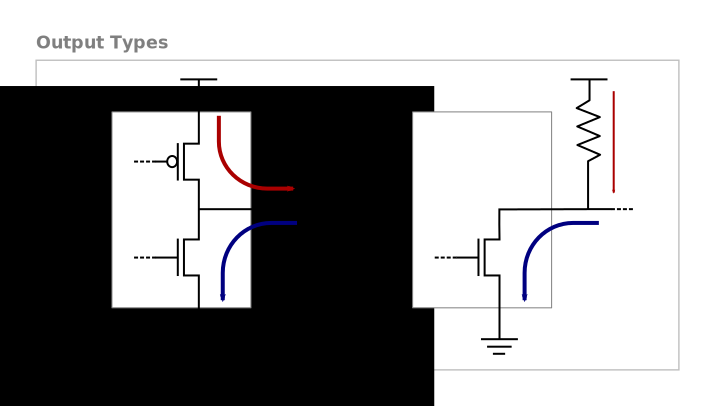
\includegraphics[width=0.75\textwidth]{output_types}
            \caption{Push-Pull \& Open-Drain Output Circuitry}
            \label{output_circuit}
        \end{figure}
        
        \subsubsection{Push-Pull vs Open Drain Outputs}
        Figure \ref{output_circuit} shows a simplified representation of the circuity for \textit{push-pull} and \textit{open-drain} outputs. 
        
        Push-Pull Outputs have drive transistors that allow the device to push the output line ``high'' by connecting to the supply rail of the device, as well as pulling it ``low'' by connecting to ground. A push-pull output can source or sink current depending on the voltage of the external system. 
        
        Open-Drain Outputs have a single transistor and can only pull the output to a low state. Because of this, open-drain systems require an external influence such as a pull-up resistor to return the line to a high state when no device is pulling it low. 
        
        \subsubsection{Why Open-Drain for I\textsuperscript{2}C}
            I\textsuperscript{2}C uses open-drain outputs due to the bi-directional nature of its signal lines. Consider a push-pull connection where two devices are attempting to output different states onto a single wire. One device attempts to drive the line high by connecting to the supply rail, while the other connects to ground to drive the line low. In this event, the two devices generate a high current power-ground short circuit, likely damaging the transistors within both devices. 
            
            Open-drain systems inherently cannot cause damaging faults because all devices can only pull the signal line low. The pull-up resistor limits the total current flowing through the system, and the most severe error that can occur is corrupted data. 

\section{Structure of an I\textsuperscript{2}C Transaction}	
    %Briefly mention overview of data transfer & sampling.
    
    \begin{figure}[]
        \centering\includegraphics[width=\textwidth]{overview}
        \caption{Example I\textsuperscript{2}C transaction}
        \label{overview}
    \end{figure}
    
    I\textsuperscript{2}C uses a strict protocol that defines data transfer as a series of \textit{frames} and conditions.     
    Transmitted data is broken up into two types of frame: an address frame, where the master indicates the slave to which the data is sent and one or more data frames. Data is placed on the SDA line while the clock (SCL) is pulled low, and is sampled during the clock's rising edge. The time between the clock transition and data read/write is determined by the devices on the bus and the configuration of the I\textsuperscript{2}C peripheral. An example I\textsuperscript{2}C transaction is shown in figure \ref{overview}. 
    
    \subsection{Address Frame}
        \subsubsection{Start Condition}
        A master device initiates an address frame by pulling SDA low while leaving SCL high. This state, known as the \textit{start condition}, notifies all other devices that a transmission is about to begin. If two master devices concurrently attempt to take control of the bus, whichever device pulls SDA low first or transmits a lower slave address  wins the arbitration. 
        \subsubsection{Addressing and the Read/Write Bit}
        Typical I\textsuperscript{2}C addresses are 7-bits. However, some devices support an extended mode allowing for 10-bit addressing. Addresses are transmitted most significant bit (MSB) first, followed by a read/write bit indicating whether the master intends to read (1) or write (0) data to the slave device. 
        \subsubsection{Slave Acknowledgment}
        The final bit in all frames is the \textit{acknowledge} (ACK) bit. After completing the address or data bits of a frame, the transmitting device allows SDA to return high and waits for the receiver to respond by pulling it low. If this does not occur, indicating a \textit{not-acknowledge} or NACK condition, the transmitter can assume that the data was not received. 
    \subsection{Data Frame}
        \subsubsection{Data Byte}
        An I\textsuperscript{2}C transaction can contain an arbitrary number of data frames, where each frame contains a single data byte. The master device generates clock transitions on the SCL line while either the master or slave device places data on the SDA line according to the direction indicated by the read/write bit. 
        \subsubsection{Stop Condition}
        After completing the entire transaction, the master generates a \textit{stop condition} and signals the release of the bus. Stop conditions are indicated by a low to high transition of SDA, while the clock (SCL) remains high. During normal data transfer, SDA only changes state while the SCL signal is low. 
        \subsubsection{Restart Condition}
        Because I\textsuperscript{2}C is a half-duplex bus, master and slave devices can not transmit simultaneously. If a master wishes to both write and read from a slave, it must begin a new transaction with the read/write bit set correctly. 
        
        In the case where chained transactions are desired, ending the current transaction with a stop condition would release the bus and allow other devices to steal control before the master begins again. To prevent this, devices are allowed to issue new start conditions without properly ending the previous transaction with a stop. This event is known as a \textit{restart} condition. 

\section{Using the I\textsuperscript{2}C Peripheral}
    The I\textsuperscript{2}C peripheral in the STM32F0 has a high-level interface that hides much of the complexity of the bus protocol. The peripheral can automatically generate a complete I\textsuperscript{2}C transaction once the user configures basic parameters such as the slave address and number of bytes to transfer. 
    
    While this interface is simpler than the original protocol, the user must be careful when initializing the peripheral. The I\textsuperscript{2}C peripherals in the STM32F0 support a variety of modes and speeds. Due to the strictness of the I\textsuperscript{2}C standard, incorrectly configured settings may prevent slave devices from responding.

\subsection{Peripheral Registers}
    \subsubsection{Control Register 1 (I2C\_CR1)}
    The control register 1 manages the overall operation of the I\textsuperscript{2}C peripheral. These settings fall into a few different categories:
    \begin{itemize}
        \item \textbf{SMBus Configuration} -- SMBus is a more restrictive protocol designed for greater reliability than conventional I\textsuperscript{2}C. Configuration bits and registers related to SMBus should be left at default. 
        \item \textbf{Slave Mode Configuration} -- The I\textsuperscript{2}C peripheral operates as both a slave and master device. Since we won't be using a multi-master network for this lab, these settings can be ignored. 
        \item \textbf{Noise Filters} -- The I\textsuperscript{2}C peripheral has both analog and digital noise filters. The analog filter is enabled by default and is sufficient for normal operation. 
        \item \textbf{Interrupt Enables} -- There are many I\textsuperscript{2}C conditions that can generate interrupts. This register controls interrupts for events such as transmission errors, completed transmissions, and when the bus is free. 
        \item \textbf{Peripheral Enable} -- The I\textsuperscript{2}C peripheral must be enabled in this register after it is initialized. Many initialization settings are protected once this bit is enabled.
    \end{itemize}  
    
    \subsubsection{Control Register 2 (I2C\_CR2)}
    The control register 2 contains settings for the current I\textsuperscript{2}C transaction. As such, this register is used whenever communicating with a slave device. Understanding this register is critical to using the peripheral; bits that will be used heavily during the lab exercises are described here. 
    \begin{itemize}
        \item \textbf{AUTOEND} -- When set, the peripheral will automatically generate a stop condition at the end of a transaction. This setting is undesirable when performing chained writes and reads as will be required in the lab assignment. 
        \item \textbf{NBYTES[7:0]} -- This group of 8-bits set the number of bytes to transmit in the next transaction. These must be modified using bitwise operations to prevent overwriting the rest of the register. 
        \item \textbf{STOP \& START} -- These bits generate start and stop conditions on the bus. The user starts a new transaction by writing to the START bit.
        \item \textbf{RD\_WRN} -- This bit sets the direction of data transfer for the next transaction. Its state controls the read/write bit sent in the address frame. 
        \item \textbf{SADD[9:0]} -- This group of 10-bits sets the slave address used in the next transaction. Unfortunately, the default 7-bit addressing mode uses bits [7:1] within the center of the bit field, often leading to an easy user error when learning the peripheral. These must be modified using bitwise operations to prevent overwriting the rest of the register.  
    \end{itemize}
    
    
    \subsubsection{Timing Register (I2C\_TIMINGR)}
    The I\textsuperscript{2}C peripheral has a very flexible timing system which allows the user to specify slew-rates and sampling delays. These settings can adjust the peripheral to operate reliably under non-ideal conditions. The configurable timings for the peripheral are:
    
    \begin{itemize}
        \item \textbf{PRESC} -- This field sets the prescaler used by internal timers within the I\textsuperscript{2}C peripheral. These timers generate the clock signal and control when data is sampled.  
        \item \textbf{SCLL \& SCLH} -- These fields set the high and low periods of the clock signal (SCL). Because these can be set independently, the peripheral allows the user to specify an asymmetric clock. 
        \item \textbf{SDADEL \& SCLDEL} -- These fields determine the data setup and hold timing used when transmitting and receiving. 
    \end{itemize}

    \subsubsection{Interrupt and Status Register (I2C\_ISR)}
    The read-only interrupt and status register indicates the state of every interrupt condition in the peripheral. These flag bits are also used by blocking drivers to determine the state of the bus.
    
    The peripheral hardware clears many of these flags automatically whenever the appropriate action is completed by the user. The documentation should always be examined to determine the specific conditions required for each bit. 
    \subsubsection{Interrupt Clear Register (I2C\_ICR)}
    The interrupt clear register is used to clear status flags that require direct acknowledgment from the user. Many of these involve error condition interrupts, and will not be used in the lab assignment.
    
    \subsubsection{Transmit \& Receive Data Registers (I2C\_TXDR{\textbackslash}I2C\_RXDR)}
    These registers are written and read by the user application during use of the peripheral. 
    
    \subsubsection{Other Peripheral Registers}
    The I\textsuperscript{2}C peripheral has additional registers used by the slave and SMBus modes. These should be left in their default state.

\subsection{Initializing the Peripheral} \label{i2c_init}
   
    The I\textsuperscript{2}C peripherals in the STM32F0 offer a variety of operating modes, and have a large set of status flags used for developing interrupt based non-blocking drivers. Depending on the modes and interrupts used, the initialization of the peripheral can be complex or relatively simple. The complete initialization process is documented in section 26.4.5 of the peripheral reference manual. 
    
    This lab requires only the I\textsuperscript{2}C master mode using blocking operations; these involve minimal initialization and can be configured by the following steps.
    
    \begin{itemize}
        \item Enable and configure the GPIO output pins used by the I\textsuperscript{2}C peripheral to alternate function mode.
        \begin{itemize}
            \item Set the pin's output type to be \underline{\textit{open-drain}} in the GPIOx\_OTYPER register. 
            \item Set the appropriate alternate function number in the GPIOx\_AFR registers. 
        \end{itemize}
        \item Enable the I\textsuperscript{2}C system clock using the RCC peripheral.
        \item Configure bus timing using the I2Cx\_TIMINGR.
        \item Enable the I\textsuperscript{2}C peripheral using the PE bit in the CR1 register.
    \end{itemize} 
     
    \subsubsection{Configuring the Bus Timing}
    The only system-wide initialization step used by the basic modes in this lab is to set the I\textsuperscript{2}C timing register. The values within this register determine the transmission rate of the interface. 
    
    The flexibility of the STM32F0's I\textsuperscript{2}C timing system allows for fine-tuned operation. However, this flexibility requires the user to derive timing constants from series of equations documented in the peripheral manual. 
    
    Fortunately, section 26.4.10 contains tables of pre-calculated parameters which result in standard behavior suitable for most systems. Figure \ref{timing} shows the timing table for the default 8MHz processor speed. The columns within this table represent the supported  I\textsuperscript{2}C speed modes. Configuring the bit fields in the TIMINGR to these values provides acceptable performance.  

    \begin{figure}[]
        \centering\includegraphics[width=\textwidth]{timing}
        \caption{Timing table for the default 8MHz processor speed}
        \label{timing}
    \end{figure}

    \subsubsection{Enabling the Peripheral}
    Before the I\textsuperscript{2}C interface can be used the peripheral enable (PE) bit must be set in the CR1 register. Setting this bit locks all of the system-wide configuration bits and registers to prevent accidental modification during transmission. Clearing the PE bit after it has been set performs a peripheral reset and clears all configuration registers. 
    
    Transaction specific options found in the CR2 register are not locked by the PE bit. These are modified at the beginning of each transaction to set parameters such as the slave address.

\subsection{Basic Communication} \label{i2c_comm}
    The processes of writing and reading from a slave device are very similar. Every communication follows a few simple steps: setting transaction parameters, starting the peripheral, waiting on status flags, and looping to previous steps depending on the flags set and length of data. Figure \ref{trans_flow} contains a flowchart demonstrating the general process of using the master mode with blocking operations. 

    \subsubsection{Setting up the Transaction}
        Each I\textsuperscript{2}C transaction is initialized by completing the following steps in the CR2 register:
        \begin{enumerate}
            \item Set the slave address in the SADD[7:1] bit field. 
            \item Set the number of data byte to be transmitted in the NBYTES[7:0] bit field.
            \item Configure the RD\_WRN to indicate a read/write operation.
            \item Do not set the AUTOEND bit, this lab requires software start/stop operation. 
            \item Setting the START bit to begin the address frame. 
        \end{enumerate}
    
    \begin{warning}
        Set the START bit in the CR2 register \underline{after} configuring the slave address and transaction length. Similar to how the PE bit locks system-wide configurations, setting the START bit locks the transaction parameters until the peripheral has completed the address frame. 
    \end{warning}
    
    \begin{example}[Setting the SADD and NBYTES Bit Fields]
       
        Since the SADD and NBYTES bit fields are not within separate registers, they cannot be directly assigned without overwriting the remainder of the CR2 register. Because of this, bitwise operations are required to clear and set the bit fields. 
        
        Rather than directly assigning each bit, it is helpful to use the desired value as a shifted bitmask directly. The following example demonstrates how to clear and set these bit fields using bitwise operations. 
        %\code{./Files/setup.c}{Setting the SADD and NBYTES bit fields using bitwise operations}{setup}
        
         \smallskip
         \colorbox{gray!20!white}{
             \parbox{\linewidth-2\fboxsep} {
                 \centering 
                 \lstinputlisting[language=C]{./Files/setup.c}
             }
         }
     
         \smallskip
    \end{example}
    
    \subsubsection{Transmitting to a Slave Device}
        Once a transaction has been initiated, the driver must wait until the I\textsuperscript{2}C peripheral has transmitted the address frame and received an acknowledgment from the slave device. This is accomplished by polling on both the \textit{Transmit Interrupt Status} (TXIS) and \textit{Not Acknowledge Received Flag} (NACKF) status bits. 
        
        Depending on which flag bit is set determines the following operation:
        \begin{itemize}
            \item \textbf{NACKF Flag Set} -- This flag indicates that the slave device did not acknowledge the address frame. There is likely a configuration issue; the current transaction has been aborted. Clear the NACKF flag, revise the initialization, and attempt to start a new transaction. 
            \item \textbf{TXIS Flag Set} -- The address frame completed successfully, and the peripheral is requesting new data to be written into the transmit data (TXDR) register. 
        \end{itemize}
        
        Once successfully transmitting data, repeat the polling and writing process with the NACKF and TXIS bits until the number of bytes in the NBYTES bit field has been written. After reaching this limit, poll instead on the \textit{Transfer Complete} (TC) status flag. 
        
        The TC flag is set when the peripheral determines that the transaction is complete, and is waiting for the user to perform a restart or stop condition. To restart, return to the top of the process for transmitting or receiving data from the slave. To release the bus by issuing a stop condition, set the STOP bit in the CR2 register.  
    
    \subsubsection{Receiving from a Slave Device}
        Receiving from a slave device is nearly identical to transmitting. Often, receive transactions occur as a restart of a transmit. This is because many slave devices operate using a register-based control scheme similar to using peripheral registers. The difference is that to access the registers within a slave device, the user first transmits the register address to select for the follow-up read operation. \\
        
        Once the transaction is initiated, the driver should poll on the \textit{Receive Data Register Not Empty} (RXNE) and \textit{Not Acknowledge Received Flag} (NACKF) status bits. Assuming that no acknowledgment errors occurred, the RXNE status flag indicates that data has been received and is waiting to be read from the receive data (RXDR) register.  
        
        Multi-byte reads are accomplished by repeatedly polling on the status flags. Once the number of bytes has been read as was set in the NBYTES register, the user can issue a restart or stop condition.  
    
    \begin{figure}[]
       \centering\includegraphics[width=\textwidth]{trans_flow}
       \caption{Blocking transmit and receive flowchart}
       \label{trans_flow}
    \end{figure}

\section{Using the L3GD20 Digital Gyroscope}
Gyroscopic sensors measure angular velocity (rate/speed of rotation) in degrees per second. The L3GD20 is a three-axis digital-output device, which returns positive values for counter-clockwise rotation, negative for clockwise, and near zero when not in motion. Figure \ref{gyro_axis} shows the orientation of the different axises and how they transition to the Discovery board. The axises can also be oriented by examining the pin 1 marking (engraved dot) on the top of the sensor packaging.  

The L3GD20 has the capability to communicate over both SPI (serial-peripheral-interface) and I2C. The interface used is selected by the state of one of the connecting pins on the chip. 

The datasheet for the L3GD20 digital gyroscope can be downloaded from ST's website using the following link: \href{http://www.st.com/resource/en/datasheet/l3gd20.pdf}{\textbf{(L3GD20 Datasheet) l3gd20.pdf}}

\begin{figure}[]
    \centering\includegraphics[width=\textwidth]{gyro_axis}
    \caption{Gyroscope axis orientation.}
    \label{gyro_axis}
\end{figure}

\subsection{Device Registers}
Similar to the internal peripherals of the STM32F0, the L3GD20 device has a set of registers which configure its operating parameters. When starting a transaction with the sensor, the first written byte is always the address of a device register to select for the read/write operation. Figure \ref{gyro_flow} contains high-level flowcharts for reading and writing registers. 

\begin{figure}[]
    \centering\includegraphics[width=\textwidth]{gyro_flow}
    \caption{Register read/write flowcharts.}
    \label{gyro_flow}
\end{figure}


\subsubsection{Chip ID Register (WHO\_AM\_I)}
Most devices contain an ID register with a known value documented in the datasheet. The primary purpose of the ID register is to provide something to compare against when testing driver code for the device. 
\begin{itemize}
    \item Address: 0x0F
    \item Should contain the value: 0xD4
\end{itemize}

\subsubsection{Control Register 1 (CTRL\_REG1)}
The control register 1 enables the axises of the sensor and sets the output bandwidth and data-rate. 
\begin{itemize}
    \item Address: 0x20
\end{itemize}

\subsubsection{Status Register (STATUS\_REG)}
The status register indicates whether new data has been produced by the sensor and is ready to be accessed. It also contains overrun error flags which indicate that previous data was overwritten before it was read. Many of these events can be configured to produce interrupt requests on the two interrupt output pins of the chip.
\begin{itemize}
    \item Address: 0x27
\end{itemize}

\subsubsection{X-Axis Data Registers (OUT\_X\_L \& OUT\_X\_H)}
The L3GD20 produces 16-bit signed data for each axis. The two 8-bit registers for each axis must be shifted and bitwise OR'd together to produce the actual sensor output. These registers contain the x-axis data. 
\begin{itemize}
    \item OUT\_X\_L (Data Low Bytes) Address: 0x28 (0xA8 when reading both registers in same transaction)
    \item OUT\_X\_H (Data High Bytes) Address: 0x29
    \item These registers should be read together in the same transaction. When reading multiple bytes, the L3GD20 automatically advances to the next register if the highest bit was set in the first address. 
\end{itemize} 

\subsubsection{Y-Axis Data Registers (OUT\_Y\_L \& OUT\_Y\_H)}
These registers contain the 16-bit y-axis data. 
\begin{itemize}
    \item OUT\_X\_L (Data Low Bytes) Address: 0x2A (0xAA when reading both registers in same transaction)
    \item OUT\_X\_H (Data High Bytes) Address: 0x2B
    \item These registers should be read together in the same transaction. When reading multiple bytes, the L3GD20 automatically advances to the next register if the highest bit was set in the first address. 
\end{itemize}

\subsubsection{Other Device Registers}
This lab uses the most basic methods of collecting data from the sensor. The L3GD20 has many advanced features such multi-mode FIFO buffers, low and high-pass filters, interrupt triggers, and threshold compare. Because of these unused features, there are multiple control registers not mentioned in this manual. These features are disabled by default and their control registers should be left in their reset/default state.


\subsection{Device Connections}
Since the L3GD20 can operate using both I2C and SPI, the device pins serve multiple purposes depending on the selected mode. The Discovery board originally intended that the sensor be interfaced using SPI. This complicates the connections slightly, you will need to use a few jumper wires between pins on the Discovery board in order to use the sensor with I2C. 

Because the I2C clock and data lines require external pull-up resistors, you will need to attach resistors within the range of 4.7 to 10 kOhm between these lines to the 3V source pin on the discovery board. While in the lab, your lab aide should have pull-up cables available for use with 10 kOhm resistors built-in.  

Figure \ref{gyro_pins} is a portion of the L3GD20 pinout and signal description table. In order to correctly connect these signals to the STM32F072 it is necessary to trace them through the Discovery board manual. Because the actual use of I2C is expected to take a significant amount of time in this lab, the exercises will indicate what GIPO pins and their modes to use.  


\begin{figure}[]
    \centering\includegraphics[width=\textwidth]{gyro_pins}
    \caption{Partial L3GD20 pinout and signal description table.}
    \label{gyro_pins}
\end{figure}

%\begin{itemize}
%    \item \textbf{SCL/SPC}
%    \begin{itemize}
%        \item This pin acts as the I2C (SCL) or SPI (SCK) clock signal.
%        \item Connected to pin PB13 on the STM32F072
%        \item This pin requires an external 10 kOhm pull-up resistor to the 3V pin on the Discovery board. 
%    \end{itemize}
%    \item \textbf{SDA/SDI/SDO}
%    \begin{itemize}
%        \item 
%    \end{itemize}
%\end{itemize}


\section{Lab Assignment}
Within this lab's exercises you will be using I2C to communicate between the STM32F072 and the L3GD20 digital gyroscope sensor. The first exercise involves reading a single register to familiarize you with the basic concepts of writing and reading over I2C. The second exercise initializes and reads measured data from the sensor to  implement a rotation indicator using the LEDs on the discovery board. 

Communicating over I2C can be very tricky unless you are comfortable with the interface and peripheral. It is very likely that you will have trouble getting your code to work properly on the first attempt. Using a logic analyzer with the I2C decoder will be very helpful as you will be able to see the different conditions of the bus and whether the transaction is progressing successfully. 

When using the logic analyzer, you will want to primarily observe the SDA and SCL signals. Place a falling-edge trigger on the line used for the SCL signal. The default state of the I2C lines is high, and the clock will drop when the peripheral first signals the start condition.  

Because the operation of the I2C peripheral takes some care, the lab exercises will provide instructions on what pins to connect as well as the GPIO configuration. 

\subsection{Reading the L3GD20 ``WHO\_AM\_I'' Register}
\subsubsection{Connecting The Sensor Pins}
Because the Discovery board is designed to use the SPI interface to connect to the sensor, some minor rewiring is necessary. Your lab aide should provide pull-up cables and jumper wires for in-lab use. Outside the scheduled lab sessions, you may need to provide your own jumpers and pull-up resistors. 

The lab provided pull-up cables have three ends. One black/gray and two of a random matching color. The black/gray and colored ends are connected with 10 kOhm resistors. 

\begin{enumerate}
    \item Connect pull-up resistors to the I2C SCL and SDA pins. 
    \begin{itemize}
        \item Connect the black/gray end of the provided pull-up cable to the \textbf{3V} power pin on the upper-left corner of the Discovery board.
        \item Connect one colored end to PB15 (L3GD20 SDA pin).
        \item Connect the other colored end to PB13 (L3GD20 SCL pin).
    \end{itemize}
    \item Connect the STM32F072 SDA pin to the L3GD20 SDA pin.
    \begin{itemize}
        \item Use a jumper wire to connect PB11 to PB15.
        \item It might be helpful to remember that the pins on the Discovery board can be connected from both sides of the board. 
    \end{itemize}
\end{enumerate}

\subsubsection{Setting the GPIO Modes}
Aside from the SCL and SDA pins, the L3GD20 requires additional signals to set the interface mode and slave address. Pin PC0 is connected to the SPI/I2C mode select pin, and PB14 controls the slave address when in I2C mode. 

\begin{enumerate}
    \item Enable GPIOB and GPIOC in the RCC. 
    \item Set PB11 to alternate function mode, open-drain output type, and select I2C2\_SDA as its alternate function.
    \item Set PB13 to alternate function mode, open-drain output type, and select I2C2\_SCL as its alternate function.
    \item Set PB14 to output mode, push-pull output type, and initialize/set the pin high.
    \item Set PC0 to output mode, push-pull output type, and initialize/set the pin high.
\end{enumerate}

\begin{warning}
    Ensure that PB11 and PB13 are set to \textbf{open-drain} output type. Otherwise, the I2C slave will not be able to respond during communication. Leave PB15 in input mode since it is connected to PB11 through a jumper wire. Modifying the mode of pin PB15 could cause a conflict if the two pins try to output different logic states. 
\end{warning}

\subsubsection{Initializing the I2C Peripheral}
In this lab we will be using only the basic operation of the I2C peripheral. Because of this, most of the control bits can be left in their default state. You will only need to modify the few registers listed in the lab manual. 

\begin{enumerate}
    \item Enable the I2C2 peripheral in the RCC.
    \begin{itemize}
        \item The I2C2 peripheral is simpler and requires less configuration than I2C1.
    \end{itemize}
    \item Set the parameters in the TIMINGR register to use 100 kHz standard-mode I2C. 
    \begin{itemize}
        \item See section \ref{i2c_init} and figure \ref{timing} in this lab manual.
        \item You will need to shift the parameter values into the proper bit-location and use bitwise operators to apply them to the register. 
    \end{itemize}
    \item Enable the I2C peripheral using the PE bit in the CR1 register. 
\end{enumerate}

\subsubsection{Reading the Register}
Figure \ref{trans_flow} shows a complete flowchart indicating the steps and actions required to perform blocking reads and writes to an I2C device. However, in this exercise, each step will be listed as a complete walk-through of the process of performing a basic I2C transaction. 

For debugging purposes you may want to set LED patterns or print USART messages as you advance through the different portions.

\begin{enumerate}
    \item Set the transaction parameters in the CR2 register. (See section \ref{i2c_comm})
    \begin{itemize}
        \item \textbf{Set the L3GD20 slave address = 0x6B}
        \begin{itemize}
            \item The slave address is documented in the I2C section of the sensor datasheet. It is modified by the state of the SDO pin.
        \end{itemize}
        \item Set the number of bytes to transmit = 1.
        \item Set the RD\_WRN bit to indicate a \underline{\textit{write}} operation.
        \item Set the START bit.
    \end{itemize}
    \item Wait until either of the TXIS (Transmit Register Empty/Ready) or NACKF (Slave Not-Acknowledge) flags are set.
    \begin{itemize}
        \item If the NACKF flag is set, the slave did not respond to the address frame. You may have a wiring or configuration error. 
        \item Continue if the TXIS flag is set. 
    \end{itemize}
    \item Write the address of the ``WHO\_AM\_I'' register into the I2C transmit register. (TXDR)
    \item Wait until the TC (Transfer Complete) flag is set.
    \item Reload the CR2 register with the same parameters as before, but set the RD\_WRN bit to indicate a \underline{\textit{read}} operation.
    \begin{itemize}
        \item Don't forget to set the START bit again to perform a I2C restart condition.
    \end{itemize}
    \item Wait until either of the RXNE (Receive Register Not Empty) or NACKF (Slave Not-Acknowledge) flags are set.
    \begin{itemize}
        \item Continue if the RXNE flag is set. 
    \end{itemize}
    \item Check the contents of the RXDR register to see if it matches 0xD4. (expected value of the ``WHO\_AM\_I'' register) 
    \item Wait until the TC (Transfer Complete) flag is set.
    \item Set the STOP bit in the CR2 register to release the I2C bus.
\end{enumerate}

After successfully verifying that the ``WHO\_AM\_I'' register matches the expected value, include a logic analyzer screenshot of the I2C transaction in your postlab.
 
\subsection{Using the L3GD20 to Implement a Rotation Indicator}
Now that you have completed basic reading and writing to the sensor, it is time to enable and use the data it produces. Since this lab is teaching basic I2C and not how to control the L3GD20 gyro effectively, you aren't required to fully initialize the device to use the FIFO buffer and other features.

In this section you will be repeatedly reading the sensor's data registers within the main \texttt{while} loop of your program. Because the sensor only produces data at a defined rate (95 Hz default) you will want to introduce some delay between reads.

Unlike the STM32F0 internal peripherals, you typically won't perform read-modify-write operations on remote device registers. Instead, directly calculate the desired bit pattern and overwrite the entire register. If your device doesn't appear to be operating correctly regardless of correct I2C transactions, you may want to perform a verification read after writing to check if things were written to the values you intended. 

\subsubsection{Initializing the Gyroscope}
Because we are polling the sensor in its basic mode, the only initialization step is to enable the axises and bring the device out of power-down mode. This exercise doesn't provide step-by-step instructions on how to read and write to the required registers. You will want to refer to the flowcharts in figures \ref{trans_flow} and \ref{gyro_flow}.

\begin{enumerate}
    \item Enable the X and Y sensing axis in the CTRL\_REG1 register.
    \item Set the sensor into ``normal or sleep mode'' using the PD bit in the CTRL\_REG1 register.
    \item All other bits in the CTRL\_REG1 register should be set to 0. These place the device in the default low-speed mode.
\end{enumerate} 

All other control registers enable advanced features such as the FIFO, interrupt and filter systems. Unless you have the base system operating, don't attempt to enable and use these. 

\subsubsection{Exercise Specifications}
You will need to implement an application that fulfills the following requirements:
\begin{enumerate}
    \item Initialize the L3GD20 gyroscope sensor to read the X and Y axises.
    \item Read and save the value of the X and Y axis data registers every 100 ms.
    \begin{itemize}
        \item You will need to assemble the 16-bit measured value from the two data registers for each axis. 
    \end{itemize}
    \item Use the four LEDs to indicate whether each measured axis is positive or negative. 
    \begin{itemize}
        \item Because of measurement noise and to prevent the lights from triggering due to small vibrations, set a minimum threshold before changing the active LED.
        \item Design your application such that the LED nearest the direction of rotation lights up.
        \begin{itemize}
            \item For example: Light the orange LED when the board is rotated/tilted in the positive X-axis direction. Refer to figure \ref{gyro_axis} for axis orientation. 
        \end{itemize} 
    \end{itemize}
\end{enumerate}

\begin{warning}
    Most I2C devices will automatically advance to the next register when you attempt to read multiple data bytes. The L3GD20 also contains this feature, but it \underline{must be explicitly requested} when writing the starting register address. 
    
    In order to read multiple bytes, it is necessary to set the most significant bit of the starting register address. Otherwise the device will repeatedly send the same register data for each byte requested.
\end{warning}

\end{document}
